% Options for packages loaded elsewhere
\PassOptionsToPackage{unicode}{hyperref}
\PassOptionsToPackage{hyphens}{url}
%
\documentclass[
]{book}
\usepackage{lmodern}
\usepackage{amssymb,amsmath}
\usepackage{ifxetex,ifluatex}
\ifnum 0\ifxetex 1\fi\ifluatex 1\fi=0 % if pdftex
  \usepackage[T1]{fontenc}
  \usepackage[utf8]{inputenc}
  \usepackage{textcomp} % provide euro and other symbols
\else % if luatex or xetex
  \usepackage{unicode-math}
  \defaultfontfeatures{Scale=MatchLowercase}
  \defaultfontfeatures[\rmfamily]{Ligatures=TeX,Scale=1}
\fi
% Use upquote if available, for straight quotes in verbatim environments
\IfFileExists{upquote.sty}{\usepackage{upquote}}{}
\IfFileExists{microtype.sty}{% use microtype if available
  \usepackage[]{microtype}
  \UseMicrotypeSet[protrusion]{basicmath} % disable protrusion for tt fonts
}{}
\makeatletter
\@ifundefined{KOMAClassName}{% if non-KOMA class
  \IfFileExists{parskip.sty}{%
    \usepackage{parskip}
  }{% else
    \setlength{\parindent}{0pt}
    \setlength{\parskip}{6pt plus 2pt minus 1pt}}
}{% if KOMA class
  \KOMAoptions{parskip=half}}
\makeatother
\usepackage{xcolor}
\IfFileExists{xurl.sty}{\usepackage{xurl}}{} % add URL line breaks if available
\IfFileExists{bookmark.sty}{\usepackage{bookmark}}{\usepackage{hyperref}}
\hypersetup{
  pdftitle={A Minimal Book Example},
  pdfauthor={Yihui Xie},
  hidelinks,
  pdfcreator={LaTeX via pandoc}}
\urlstyle{same} % disable monospaced font for URLs
\usepackage{color}
\usepackage{fancyvrb}
\newcommand{\VerbBar}{|}
\newcommand{\VERB}{\Verb[commandchars=\\\{\}]}
\DefineVerbatimEnvironment{Highlighting}{Verbatim}{commandchars=\\\{\}}
% Add ',fontsize=\small' for more characters per line
\usepackage{framed}
\definecolor{shadecolor}{RGB}{248,248,248}
\newenvironment{Shaded}{\begin{snugshade}}{\end{snugshade}}
\newcommand{\AlertTok}[1]{\textcolor[rgb]{0.94,0.16,0.16}{#1}}
\newcommand{\AnnotationTok}[1]{\textcolor[rgb]{0.56,0.35,0.01}{\textbf{\textit{#1}}}}
\newcommand{\AttributeTok}[1]{\textcolor[rgb]{0.77,0.63,0.00}{#1}}
\newcommand{\BaseNTok}[1]{\textcolor[rgb]{0.00,0.00,0.81}{#1}}
\newcommand{\BuiltInTok}[1]{#1}
\newcommand{\CharTok}[1]{\textcolor[rgb]{0.31,0.60,0.02}{#1}}
\newcommand{\CommentTok}[1]{\textcolor[rgb]{0.56,0.35,0.01}{\textit{#1}}}
\newcommand{\CommentVarTok}[1]{\textcolor[rgb]{0.56,0.35,0.01}{\textbf{\textit{#1}}}}
\newcommand{\ConstantTok}[1]{\textcolor[rgb]{0.00,0.00,0.00}{#1}}
\newcommand{\ControlFlowTok}[1]{\textcolor[rgb]{0.13,0.29,0.53}{\textbf{#1}}}
\newcommand{\DataTypeTok}[1]{\textcolor[rgb]{0.13,0.29,0.53}{#1}}
\newcommand{\DecValTok}[1]{\textcolor[rgb]{0.00,0.00,0.81}{#1}}
\newcommand{\DocumentationTok}[1]{\textcolor[rgb]{0.56,0.35,0.01}{\textbf{\textit{#1}}}}
\newcommand{\ErrorTok}[1]{\textcolor[rgb]{0.64,0.00,0.00}{\textbf{#1}}}
\newcommand{\ExtensionTok}[1]{#1}
\newcommand{\FloatTok}[1]{\textcolor[rgb]{0.00,0.00,0.81}{#1}}
\newcommand{\FunctionTok}[1]{\textcolor[rgb]{0.00,0.00,0.00}{#1}}
\newcommand{\ImportTok}[1]{#1}
\newcommand{\InformationTok}[1]{\textcolor[rgb]{0.56,0.35,0.01}{\textbf{\textit{#1}}}}
\newcommand{\KeywordTok}[1]{\textcolor[rgb]{0.13,0.29,0.53}{\textbf{#1}}}
\newcommand{\NormalTok}[1]{#1}
\newcommand{\OperatorTok}[1]{\textcolor[rgb]{0.81,0.36,0.00}{\textbf{#1}}}
\newcommand{\OtherTok}[1]{\textcolor[rgb]{0.56,0.35,0.01}{#1}}
\newcommand{\PreprocessorTok}[1]{\textcolor[rgb]{0.56,0.35,0.01}{\textit{#1}}}
\newcommand{\RegionMarkerTok}[1]{#1}
\newcommand{\SpecialCharTok}[1]{\textcolor[rgb]{0.00,0.00,0.00}{#1}}
\newcommand{\SpecialStringTok}[1]{\textcolor[rgb]{0.31,0.60,0.02}{#1}}
\newcommand{\StringTok}[1]{\textcolor[rgb]{0.31,0.60,0.02}{#1}}
\newcommand{\VariableTok}[1]{\textcolor[rgb]{0.00,0.00,0.00}{#1}}
\newcommand{\VerbatimStringTok}[1]{\textcolor[rgb]{0.31,0.60,0.02}{#1}}
\newcommand{\WarningTok}[1]{\textcolor[rgb]{0.56,0.35,0.01}{\textbf{\textit{#1}}}}
\usepackage{longtable,booktabs}
% Correct order of tables after \paragraph or \subparagraph
\usepackage{etoolbox}
\makeatletter
\patchcmd\longtable{\par}{\if@noskipsec\mbox{}\fi\par}{}{}
\makeatother
% Allow footnotes in longtable head/foot
\IfFileExists{footnotehyper.sty}{\usepackage{footnotehyper}}{\usepackage{footnote}}
\makesavenoteenv{longtable}
\usepackage{graphicx,grffile}
\makeatletter
\def\maxwidth{\ifdim\Gin@nat@width>\linewidth\linewidth\else\Gin@nat@width\fi}
\def\maxheight{\ifdim\Gin@nat@height>\textheight\textheight\else\Gin@nat@height\fi}
\makeatother
% Scale images if necessary, so that they will not overflow the page
% margins by default, and it is still possible to overwrite the defaults
% using explicit options in \includegraphics[width, height, ...]{}
\setkeys{Gin}{width=\maxwidth,height=\maxheight,keepaspectratio}
% Set default figure placement to htbp
\makeatletter
\def\fps@figure{htbp}
\makeatother
\setlength{\emergencystretch}{3em} % prevent overfull lines
\providecommand{\tightlist}{%
  \setlength{\itemsep}{0pt}\setlength{\parskip}{0pt}}
\setcounter{secnumdepth}{5}
\usepackage{booktabs}
\usepackage[]{natbib}
\bibliographystyle{apalike}

\title{A Minimal Book Example}
\author{Yihui Xie}
\date{2021-04-18}

\begin{document}
\maketitle

{
\setcounter{tocdepth}{1}
\tableofcontents
}
\hypertarget{prerequisites}{%
\chapter{Prerequisites}\label{prerequisites}}

This is a \emph{sample} book written in \textbf{Markdown}. You can use anything that Pandoc's Markdown supports, e.g., a math equation \(a^2 + b^2 = c^2\).

The \textbf{bookdown} package can be installed from CRAN or Github:

\begin{Shaded}
\begin{Highlighting}[]
\KeywordTok{install.packages}\NormalTok{(}\StringTok{"bookdown"}\NormalTok{)}
\CommentTok{# or the development version}
\CommentTok{# devtools::install_github("rstudio/bookdown")}
\end{Highlighting}
\end{Shaded}

Remember each Rmd file contains one and only one chapter, and a chapter is defined by the first-level heading \texttt{\#}.

To compile this example to PDF, you need XeLaTeX. You are recommended to install TinyTeX (which includes XeLaTeX): \url{https://yihui.org/tinytex/}.

\hypertarget{intro}{%
\chapter{Basics}\label{intro}}

The sample space is the set of all possible outcomes. An event is a subset of the sample space, either an outcome (simple event) or a collection of outcomes (compound event).

Events are \textbf{independent} if an occurrence of one has no effect on the probability of the other. Events are \textbf{exclusive} if \(P(AB) = 0\). Use the multiplication rule to calculate combined probabilities for non-exclusive events (\(P(A|B) = P(A)P(B)\) for independent events, and \$P*()(), and the addition rule to calculate combined probabilities for exclusive events.

)

\hypertarget{random-variables-and-distributions}{%
\chapter{Random Variables and Distributions}\label{random-variables-and-distributions}}

\hypertarget{binomial}{%
\section{Binomial}\label{binomial}}

Binomial sampling is used to model counts of one level of a categorical variable over a \emph{fixed sample size}.

\begin{quote}
If \(X\) is the count of successful events in \(n\) identical and independent Bernoulli trials of success probability \(\pi\), then \(X\) is a random variable with a binomial distribution \(X \sim \mathrm{Bin}(n,\pi)\)

\[f(X = k;n, \pi) = \frac{n!}{k!(n-k)!} \pi^k (1-\pi)^{n-k} \hspace{1cm} k \in (0, 1, ..., n), \hspace{2mm} \pi \in [0, 1]\]

with \(E(X)=n\pi\) and \(Var(X) = n\pi(1-\pi)\).
\end{quote}

\hypertarget{example}{%
\subsubsection*{Example}\label{example}}
\addcontentsline{toc}{subsubsection}{Example}

Data set \texttt{dat} contains frequencies of high-risk drinkers vs non-high-risk drinkers in a college survey.

\begin{verbatim}
##  dat$high_risk   n   percent
##             No 685 0.5209125
##            Yes 630 0.4790875
\end{verbatim}

The MLE of \(\pi\) from the Binomial distribution is the sample mean.

\begin{Shaded}
\begin{Highlighting}[]
\NormalTok{x <-}\StringTok{ }\KeywordTok{sum}\NormalTok{(dat}\OperatorTok{$}\NormalTok{high_risk }\OperatorTok{==}\StringTok{ "Yes"}\NormalTok{)}
\NormalTok{n <-}\StringTok{ }\KeywordTok{nrow}\NormalTok{(dat)}
\NormalTok{p <-}\StringTok{ }\NormalTok{x }\OperatorTok{/}\StringTok{ }\NormalTok{n}
\KeywordTok{print}\NormalTok{(p)}
\end{Highlighting}
\end{Shaded}

\begin{verbatim}
## [1] 0.4790875
\end{verbatim}

\begin{Shaded}
\begin{Highlighting}[]
\KeywordTok{data.frame}\NormalTok{(}\DataTypeTok{events =} \KeywordTok{seq}\NormalTok{(}\DecValTok{550}\NormalTok{, }\DecValTok{700}\NormalTok{, }\DecValTok{10}\NormalTok{), }
           \DataTypeTok{pmf =} \KeywordTok{dbinom}\NormalTok{(}\KeywordTok{seq}\NormalTok{(}\DecValTok{550}\NormalTok{, }\DecValTok{700}\NormalTok{, }\DecValTok{10}\NormalTok{), n, p), }
           \DataTypeTok{cdf =} \KeywordTok{pbinom}\NormalTok{(}\KeywordTok{seq}\NormalTok{(}\DecValTok{550}\NormalTok{, }\DecValTok{700}\NormalTok{, }\DecValTok{10}\NormalTok{), n, p, }\DataTypeTok{lower.tail =} \OtherTok{TRUE}\NormalTok{)) }\OperatorTok
\KeywordTok{ggplot}\NormalTok{() }\OperatorTok{+}
\StringTok{  }\KeywordTok{geom_col}\NormalTok{(}\KeywordTok{aes}\NormalTok{(}\DataTypeTok{x =}\NormalTok{ events, }\DataTypeTok{y =}\NormalTok{ pmf)) }\OperatorTok{+}
\StringTok{  }\KeywordTok{geom_text}\NormalTok{(}\KeywordTok{aes}\NormalTok{(}\DataTypeTok{x =}\NormalTok{ events, }\DataTypeTok{label =} \KeywordTok{round}\NormalTok{(pmf, }\DecValTok{3}\NormalTok{), }\DataTypeTok{y =}\NormalTok{ pmf }\OperatorTok{+}\StringTok{ }\FloatTok{0.001}\NormalTok{),}
            \DataTypeTok{position =} \KeywordTok{position_dodge}\NormalTok{(}\FloatTok{0.9}\NormalTok{), }\DataTypeTok{size =} \DecValTok{3}\NormalTok{, }\DataTypeTok{vjust =} \DecValTok{0}\NormalTok{) }\OperatorTok{+}
\StringTok{  }\KeywordTok{geom_line}\NormalTok{(}\KeywordTok{aes}\NormalTok{(}\DataTypeTok{x =}\NormalTok{ events, }\DataTypeTok{y =}\NormalTok{ cdf}\OperatorTok{/}\DecValTok{40}\NormalTok{), }\DataTypeTok{size =} \DecValTok{1}\NormalTok{) }\OperatorTok{+}
\StringTok{  }\KeywordTok{scale_y_continuous}\NormalTok{(}\DataTypeTok{limits =} \KeywordTok{c}\NormalTok{(}\DecValTok{0}\NormalTok{, }\FloatTok{.025}\NormalTok{), }
                     \DataTypeTok{sec.axis =} \KeywordTok{sec_axis}\NormalTok{(}\OperatorTok{~}\StringTok{ }\NormalTok{. }\OperatorTok{*}\StringTok{ }\DecValTok{40}\NormalTok{, }\DataTypeTok{name =} \StringTok{"Cum Prob"}\NormalTok{)) }\OperatorTok{+}
\StringTok{  }\KeywordTok{labs}\NormalTok{(}\DataTypeTok{title =} \StringTok{"PMF and CDF of Binomial Distribution"}\NormalTok{,}
       \DataTypeTok{subtitle =} \KeywordTok{paste0}\NormalTok{(}\StringTok{"Bin("}\NormalTok{, n, }\StringTok{", "}\NormalTok{, scales}\OperatorTok{::}\KeywordTok{comma}\NormalTok{(p, }\DataTypeTok{accuracy =} \FloatTok{.01}\NormalTok{), }\StringTok{")"}\NormalTok{), }
       \DataTypeTok{x =} \StringTok{"X = k"}\NormalTok{, }\DataTypeTok{y =} \StringTok{"Density"}\NormalTok{)}
\end{Highlighting}
\end{Shaded}

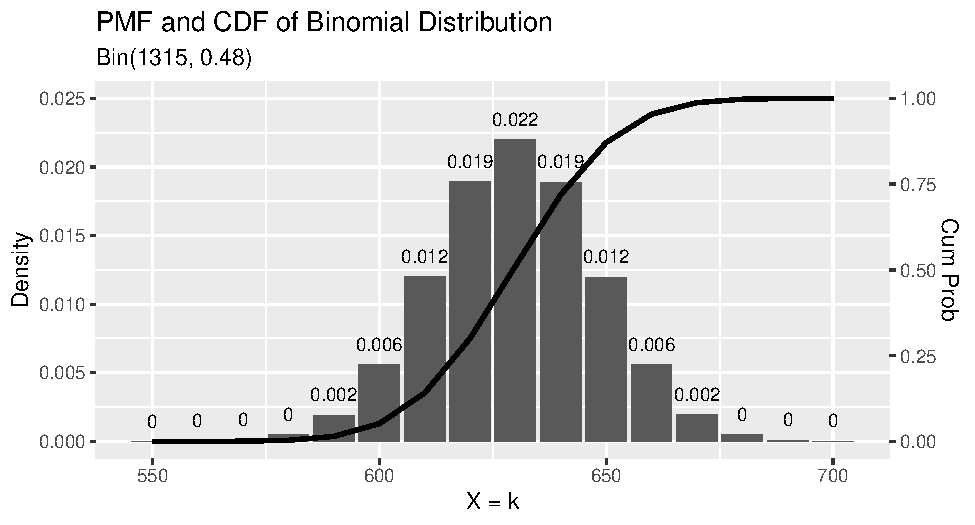
\includegraphics{probability_files/figure-latex/unnamed-chunk-5-1.pdf}

There are several ways to calculate a confidence interval for \(\pi\). One method is the \textbf{normal approximation} (Wald) interval.

\[\pi = p \pm z_{\alpha /2} \sqrt{\frac{p (1 - p)}{n}}\]

\begin{Shaded}
\begin{Highlighting}[]
\NormalTok{alpha <-}\StringTok{ }\FloatTok{.05}
\NormalTok{z <-}\StringTok{ }\KeywordTok{qnorm}\NormalTok{(}\DecValTok{1} \OperatorTok{-}\StringTok{ }\NormalTok{alpha }\OperatorTok{/}\StringTok{ }\DecValTok{2}\NormalTok{)}
\NormalTok{se <-}\StringTok{ }\KeywordTok{sqrt}\NormalTok{(p }\OperatorTok{*}\StringTok{ }\NormalTok{(}\DecValTok{1} \OperatorTok{-}\StringTok{ }\NormalTok{p) }\OperatorTok{/}\StringTok{ }\NormalTok{n)}
\NormalTok{p }\OperatorTok{+}\StringTok{ }\KeywordTok{c}\NormalTok{(}\OperatorTok{-}\NormalTok{z}\OperatorTok{*}\NormalTok{se, z}\OperatorTok{*}\NormalTok{se)}
\end{Highlighting}
\end{Shaded}

\begin{verbatim}
## [1] 0.4520868 0.5060882
\end{verbatim}

This method is easy to understand and calculate by hand, but its accuracy suffers when \(np<5\) or \(n(1-p)<5\) and it does not work at all when \(p = 0\) or \(p = 1\). Option two is the \textbf{Wilson} method.

\[\frac{p + \frac{z^2}{2n}}{1 + \frac{z^2}{n}} \pm \frac{z}{1 + \frac{z^2}{n}} \sqrt{\frac{p(1 - p)}{n} + \frac{z^2}{4n^2}}\]

\begin{Shaded}
\begin{Highlighting}[]
\NormalTok{est <-}\StringTok{ }\NormalTok{(p }\OperatorTok{+}\StringTok{ }\NormalTok{(z}\OperatorTok{^}\DecValTok{2}\NormalTok{)}\OperatorTok{/}\NormalTok{(}\DecValTok{2}\OperatorTok{*}\NormalTok{n)) }\OperatorTok{/}\StringTok{ }\NormalTok{(}\DecValTok{1} \OperatorTok{+}\StringTok{ }\NormalTok{(z}\OperatorTok{^}\DecValTok{2}\NormalTok{) }\OperatorTok{/}\StringTok{ }\NormalTok{n)}
\NormalTok{pm <-}\StringTok{ }\NormalTok{z }\OperatorTok{/}\StringTok{ }\NormalTok{(}\DecValTok{1} \OperatorTok{+}\StringTok{ }\NormalTok{(z}\OperatorTok{^}\DecValTok{2}\NormalTok{)}\OperatorTok{/}\NormalTok{n) }\OperatorTok{*}\StringTok{ }\KeywordTok{sqrt}\NormalTok{(p}\OperatorTok{*}\NormalTok{(}\DecValTok{1}\OperatorTok{-}\NormalTok{p)}\OperatorTok{/}\NormalTok{n }\OperatorTok{+}\StringTok{ }\NormalTok{(z}\OperatorTok{^}\DecValTok{2}\NormalTok{) }\OperatorTok{/}\StringTok{ }\NormalTok{(}\DecValTok{4}\OperatorTok{*}\NormalTok{(n}\OperatorTok{^}\DecValTok{2}\NormalTok{)))}
\NormalTok{est }\OperatorTok{+}\StringTok{ }\KeywordTok{c}\NormalTok{(}\OperatorTok{-}\NormalTok{pm, pm)}
\end{Highlighting}
\end{Shaded}

\begin{verbatim}
## [1] 0.4521869 0.5061098
\end{verbatim}

This is what \texttt{prop.test()} does when you set \texttt{correct\ =\ FALSE}.

\begin{Shaded}
\begin{Highlighting}[]
\KeywordTok{prop.test}\NormalTok{(}\DataTypeTok{x =}\NormalTok{ x, }\DataTypeTok{n =}\NormalTok{ n, }\DataTypeTok{correct =} \OtherTok{FALSE}\NormalTok{)}
\end{Highlighting}
\end{Shaded}

\begin{verbatim}
## 
##  1-sample proportions test without continuity correction
## 
## data:  x out of n, null probability 0.5
## X-squared = 2.3004, df = 1, p-value = 0.1293
## alternative hypothesis: true p is not equal to 0.5
## 95 percent confidence interval:
##  0.4521869 0.5061098
## sample estimates:
##         p 
## 0.4790875
\end{verbatim}

There is a second version of the Wilson interval that applies a ``continuity correction'' that aligns the ``minimum coverage probability'', rather than the ``average probability'', with the nominal value.

\begin{Shaded}
\begin{Highlighting}[]
\KeywordTok{prop.test}\NormalTok{(}\DataTypeTok{x =}\NormalTok{ x, }\DataTypeTok{n =}\NormalTok{ n)}
\end{Highlighting}
\end{Shaded}

\begin{verbatim}
## 
##  1-sample proportions test with continuity correction
## 
## data:  x out of n, null probability 0.5
## X-squared = 2.2175, df = 1, p-value = 0.1365
## alternative hypothesis: true p is not equal to 0.5
## 95 percent confidence interval:
##  0.4518087 0.5064898
## sample estimates:
##         p 
## 0.4790875
\end{verbatim}

Finally, there is the Clopper-Pearson \textbf{exact confidence interval}. Clopper-Pearson inverts two single-tailed binomial tests at the desired alpha. This is a non-trivial calculation, so there is no easy formula to crank through. Just use the \texttt{binom.test()} function and pray no one asks for an explanation.

\begin{Shaded}
\begin{Highlighting}[]
\KeywordTok{binom.test}\NormalTok{(}\DataTypeTok{x =}\NormalTok{ x, }\DataTypeTok{n =}\NormalTok{ n)}
\end{Highlighting}
\end{Shaded}

\begin{verbatim}
## 
##  Exact binomial test
## 
## data:  x and n
## number of successes = 630, number of trials = 1315, p-value = 0.1364
## alternative hypothesis: true probability of success is not equal to 0.5
## 95 percent confidence interval:
##  0.4517790 0.5064896
## sample estimates:
## probability of success 
##              0.4790875
\end{verbatim}

The expected probability of no one being a high-risk drinker is \(f(0;0.479) = \frac{1315!}{0!(1315-0)!} 0.479^0 (1-0.479)^{1315-0} = 0\).

\begin{Shaded}
\begin{Highlighting}[]
\KeywordTok{dbinom}\NormalTok{(}\DataTypeTok{x =} \DecValTok{0}\NormalTok{, }\DataTypeTok{size =}\NormalTok{ n, }\DataTypeTok{p =}\NormalTok{ p)}
\end{Highlighting}
\end{Shaded}

\begin{verbatim}
## [1] 0
\end{verbatim}

The expected probability of at least half the population being a high-risk drinker, \(f(658, 0.479)\), is impossible to write out, and slow to calculate.

\begin{Shaded}
\begin{Highlighting}[]
\KeywordTok{pbinom}\NormalTok{(}\DataTypeTok{q =} \FloatTok{.5}\OperatorTok{*}\NormalTok{n, }\DataTypeTok{size =}\NormalTok{ n, }\DataTypeTok{prob =}\NormalTok{ p, }\DataTypeTok{lower.tail =} \OtherTok{FALSE}\NormalTok{)}
\end{Highlighting}
\end{Shaded}

\begin{verbatim}
## [1] 0.06455096
\end{verbatim}

As n increases for fixed \(\pi\), the binomial distribution approaches normal distribution \(N(n\pi, n\pi(1−\pi))\). The normal distribution is a good approximation when \(n\) is large.

\begin{Shaded}
\begin{Highlighting}[]
\KeywordTok{pnorm}\NormalTok{(}\DataTypeTok{q =} \FloatTok{0.5}\NormalTok{, }\DataTypeTok{mean =}\NormalTok{ p, }\DataTypeTok{sd =}\NormalTok{ se, }\DataTypeTok{lower.tail =} \OtherTok{FALSE}\NormalTok{)}
\end{Highlighting}
\end{Shaded}

\begin{verbatim}
## [1] 0.06450357
\end{verbatim}

Suppose a second survey gets a slightly different result.

\begin{Shaded}
\begin{Highlighting}[]
\NormalTok{dat2 <-}\StringTok{ }\KeywordTok{data.frame}\NormalTok{(}
  \DataTypeTok{subject =} \DecValTok{1}\OperatorTok{:}\DecValTok{1315}\NormalTok{,}
  \DataTypeTok{high_risk =} \KeywordTok{factor}\NormalTok{(}\KeywordTok{c}\NormalTok{(}\KeywordTok{rep}\NormalTok{(}\StringTok{"Yes"}\NormalTok{, }\DecValTok{600}\NormalTok{), }\KeywordTok{rep}\NormalTok{(}\StringTok{"No"}\NormalTok{, }\DecValTok{715}\NormalTok{)))}
\NormalTok{)}
\NormalTok{(dat2_tabyl <-}\StringTok{ }\NormalTok{janitor}\OperatorTok{::}\KeywordTok{tabyl}\NormalTok{(dat2, high_risk))}
\end{Highlighting}
\end{Shaded}

\begin{verbatim}
##  high_risk   n   percent
##         No 715 0.5437262
##        Yes 600 0.4562738
\end{verbatim}

The two survey counts of \emph{high risk} = ``Yes'' are independent random variables distributed \(X \sim \mathrm{Bin}(1315, .48)\) and \(Y \sim \mathrm{Bin}(1315, .46)\). What is the probability that either variable is \(X \ge 650\)?

Let \(P(A) = P(X \le 650)\) and \(P(B) = P(Y \le 650)\). Then \(P(A|B) = P(A) + P(B) - P(AB)\), and because the events are independent, \(P(AB) = P(A)P(B)\).

\begin{Shaded}
\begin{Highlighting}[]
\NormalTok{p_a <-}\StringTok{ }\KeywordTok{pbinom}\NormalTok{(}\DataTypeTok{q =} \DecValTok{650}\NormalTok{, }\DataTypeTok{size =} \DecValTok{1315}\NormalTok{, }\DataTypeTok{prob =} \FloatTok{0.48}\NormalTok{, }\DataTypeTok{lower.tail =} \OtherTok{FALSE}\NormalTok{)}
\NormalTok{p_b <-}\StringTok{ }\KeywordTok{pbinom}\NormalTok{(}\DataTypeTok{q =} \DecValTok{650}\NormalTok{, }\DataTypeTok{size =} \DecValTok{1315}\NormalTok{, }\DataTypeTok{prob =} \FloatTok{0.46}\NormalTok{, }\DataTypeTok{lower.tail =} \OtherTok{FALSE}\NormalTok{)}
\NormalTok{p_a }\OperatorTok{+}\StringTok{ }\NormalTok{p_b }\OperatorTok{-}\StringTok{ }\NormalTok{(p_a }\OperatorTok{*}\StringTok{ }\NormalTok{p_b)}
\end{Highlighting}
\end{Shaded}

\begin{verbatim}
## [1] 0.1484061
\end{verbatim}

Here's an empirical test.

\begin{Shaded}
\begin{Highlighting}[]
\NormalTok{df <-}\StringTok{ }\KeywordTok{data.frame}\NormalTok{(}
  \DataTypeTok{x =} \KeywordTok{rbinom}\NormalTok{(}\DecValTok{10000}\NormalTok{, }\DecValTok{1315}\NormalTok{, }\FloatTok{0.48}\NormalTok{),}
  \DataTypeTok{y =} \KeywordTok{rbinom}\NormalTok{(}\DecValTok{10000}\NormalTok{, }\DecValTok{1315}\NormalTok{, }\FloatTok{0.46}\NormalTok{)}
\NormalTok{  )}
\KeywordTok{mean}\NormalTok{(}\KeywordTok{if_else}\NormalTok{(df}\OperatorTok{$}\NormalTok{x }\OperatorTok{>=}\StringTok{ }\DecValTok{650} \OperatorTok{|}\StringTok{ }\NormalTok{df}\OperatorTok{$}\NormalTok{y }\OperatorTok{>=}\StringTok{ }\DecValTok{650}\NormalTok{, }\DecValTok{1}\NormalTok{, }\DecValTok{0}\NormalTok{))}
\end{Highlighting}
\end{Shaded}

\begin{verbatim}
## [1] 0.1575
\end{verbatim}

A couple other points to remember:

\begin{itemize}
\tightlist
\item
  The Bernoulli distribution is a special case of the binomial with \(n = 1\).
\item
  The binomial distribution assumes independent trials. If you sample \emph{without replacement from a finite population}, use the hypergeometric distribution.
\end{itemize}

\hypertarget{poisson}{%
\section{Poisson}\label{poisson}}

Poisson distributions are usually used to model the number of events occurring in a fixed period of time. \href{https://towardsdatascience.com/poisson-distribution-intuition-and-derivation-1059aeab90d}{Aerin Kim} shows how the Poisson distribution is related to the binomial distribution. The key is that the binomial distribution expresses the probability of \(X = k\) events in \(n\) trials when the probability of \emph{one} event in \emph{one} trial is \(p\). Sometimes you don't know \(p\), but instead know that \(\lambda\) events occur per some time interval. You could try to back into the binomial by shrinking the time interval so that \(k\) could never be greater than one. The ratio \(p = \lambda / n\) approaches the probability of observing one event in one trial as \(n \rightarrow \infty\). As \(n \rightarrow \infty\), \(p \rightarrow 0\). If you do this and follow the math, you wind up with the Poisson distribution!

\[\begin{eqnarray}
P(X = k) &=& \mathrm{lim}_{n \rightarrow \infty} {n \choose k}p^k(1-p)^{n-k}\\
&=& \mathrm{lim}_{n \rightarrow \infty} \frac{n!}{(n-k)!k!} \left(\frac{\lambda}{n}\right)^k \left(1-\frac{\lambda}{n}\right)^{n-k}\\
&=& \mathrm{lim}_{n \rightarrow \infty} \frac{n!}{(n-k)!k!} \left(\frac{\lambda}{n}\right)^k \left(1-\frac{\lambda}{n}\right)^n\left(1-\frac{\lambda}{n}\right)^{-k}\\
&=& \mathrm{lim}_{n \rightarrow \infty} \frac{n!}{(n-k)!k!} \left(\frac{\lambda}{n}\right)^k \left(e^{-\lambda}\right)(1)\\
&=& \mathrm{lim}_{n \rightarrow \infty} \frac{n!}{(n-k)!n^k}  e^{-\lambda}\frac{\lambda^k}{k!} \\
&=& e^{-\lambda}\frac{\lambda^k}{k!}
\end{eqnarray}\]

I didn't get that last step, but I'll take it on faith.

\begin{quote}
If \(X\) is the number of successes in \(n\) (many) trials when the probability of success \(\lambda / n\) is small, then \(X\) is a random variable with a Poisson distribution \(X \sim \mathrm{Pois}(\lambda)\)

\[f(X = k;\lambda) = \frac{e^{-\lambda} \lambda^k}{k!} \hspace{1cm} k \in (0, 1, ...), \hspace{2mm} \lambda > 0\]

with \(E(X)=\lambda\) and \(\mathrm{Var}(X) = \lambda\).
\end{quote}

The Poisson distribution is also related to the exponential distribution. If the number of events per unit time follows a Poisson distribution, then the amount of time between events follows the exponential distribution.

The Poisson likelihood function is

\[L(\lambda; k) = \prod_{i=1}^N f(k_i; \lambda) = \prod_{i=1}^N \frac{e^{-\lambda} \lambda^k_i}{k_i !} = \frac{e^{-n \lambda} \lambda^{\sum k_i}}{\prod k_i}.\]

The Poisson loglikelihood function is

\[l(\lambda; k) = \sum_{i=1}^N k_i \log \lambda - n \lambda.\]

The loglikelihood function is maximized at

\[\hat{\lambda} = \sum_{i=1}^N k_i / n.\]

Thus, for a Poisson sample, the MLE for \(\lambda\) is just the sample mean.

\hypertarget{example-1}{%
\subsubsection*{Example}\label{example-1}}
\addcontentsline{toc}{subsubsection}{Example}

Data set \texttt{dat} contains frequencies of the number of goals score per match during a soccer tournament. Total goals ranged from 0 to 8.

\begin{verbatim}
##   goals freq
## 1     0   23
## 2     1   37
## 3     2   20
## 4     3   11
## 5     4    2
## 6     5    1
## 7     6    0
## 8     7    0
## 9     8    1
\end{verbatim}

The MLE of \(\lambda\) from is the sample weighted mean.

\begin{Shaded}
\begin{Highlighting}[]
\NormalTok{(lambda <-}\StringTok{ }\KeywordTok{weighted.mean}\NormalTok{(dat}\OperatorTok{$}\NormalTok{goals, dat}\OperatorTok{$}\NormalTok{freq))}
\end{Highlighting}
\end{Shaded}

\begin{verbatim}
## [1] 1.378947
\end{verbatim}

The 0.95 CI is \(\lambda \pm z_{.05/2} \sqrt{\lambda / n}\)

\begin{Shaded}
\begin{Highlighting}[]
\NormalTok{n <-}\StringTok{ }\KeywordTok{sum}\NormalTok{(dat}\OperatorTok{$}\NormalTok{freq)}
\NormalTok{z <-}\StringTok{ }\KeywordTok{qnorm}\NormalTok{(}\FloatTok{0.975}\NormalTok{)}
\NormalTok{se <-}\StringTok{ }\KeywordTok{sqrt}\NormalTok{(lambda }\OperatorTok{/}\StringTok{ }\NormalTok{n)}
\KeywordTok{paste0}\NormalTok{(}\StringTok{"["}\NormalTok{, }\KeywordTok{round}\NormalTok{(lambda }\OperatorTok{-}\StringTok{ }\NormalTok{z}\OperatorTok{*}\NormalTok{se, }\DecValTok{2}\NormalTok{), }\StringTok{", "}\NormalTok{, }\KeywordTok{round}\NormalTok{(lambda }\OperatorTok{+}\StringTok{ }\NormalTok{z}\OperatorTok{*}\NormalTok{se, }\DecValTok{2}\NormalTok{),}\StringTok{"]"}\NormalTok{)}
\end{Highlighting}
\end{Shaded}

\begin{verbatim}
## [1] "[1.14, 1.62]"
\end{verbatim}

The expected probability of scoring 2 goals in a match is \(\frac{e^{-1.38} 1.38^2}{2!}\).

\begin{Shaded}
\begin{Highlighting}[]
\KeywordTok{dpois}\NormalTok{(}\DataTypeTok{x =} \DecValTok{2}\NormalTok{, }\DataTypeTok{lambda =}\NormalTok{ lambda)}
\end{Highlighting}
\end{Shaded}

\begin{verbatim}
## [1] 0.2394397
\end{verbatim}

The expected probability of scoring 2 to 4 goals in a match is

\begin{Shaded}
\begin{Highlighting}[]
\KeywordTok{ppois}\NormalTok{(}\DataTypeTok{q =} \DecValTok{4}\NormalTok{, }\DataTypeTok{lambda =}\NormalTok{ lambda) }\OperatorTok{-}\StringTok{ }
\StringTok{  }\KeywordTok{ppois}\NormalTok{(}\DataTypeTok{q =} \DecValTok{1}\NormalTok{, }\DataTypeTok{lambda =}\NormalTok{ lambda)}
\end{Highlighting}
\end{Shaded}

\begin{verbatim}
## [1] 0.3874391
\end{verbatim}

\begin{Shaded}
\begin{Highlighting}[]
\KeywordTok{data.frame}\NormalTok{(}\DataTypeTok{events =} \DecValTok{0}\OperatorTok{:}\DecValTok{10}\NormalTok{, }
           \DataTypeTok{pmf =} \KeywordTok{dpois}\NormalTok{(}\DecValTok{0}\OperatorTok{:}\DecValTok{10}\NormalTok{, lambda), }
           \DataTypeTok{cdf =} \KeywordTok{ppois}\NormalTok{(}\DecValTok{0}\OperatorTok{:}\DecValTok{10}\NormalTok{, lambda, }\DataTypeTok{lower.tail =} \OtherTok{TRUE}\NormalTok{)) }\OperatorTok
\KeywordTok{ggplot}\NormalTok{() }\OperatorTok{+}
\StringTok{  }\KeywordTok{geom_col}\NormalTok{(}\KeywordTok{aes}\NormalTok{(}\DataTypeTok{x =} \KeywordTok{factor}\NormalTok{(events), }\DataTypeTok{y =}\NormalTok{ pmf)) }\OperatorTok{+}
\StringTok{  }\KeywordTok{geom_text}\NormalTok{(}\KeywordTok{aes}\NormalTok{(}\DataTypeTok{x =} \KeywordTok{factor}\NormalTok{(events), }\DataTypeTok{label =} \KeywordTok{round}\NormalTok{(pmf, }\DecValTok{3}\NormalTok{), }\DataTypeTok{y =}\NormalTok{ pmf }\OperatorTok{+}\StringTok{ }\FloatTok{0.01}\NormalTok{),}
            \DataTypeTok{position =} \KeywordTok{position_dodge}\NormalTok{(}\FloatTok{0.9}\NormalTok{), }\DataTypeTok{size =} \DecValTok{3}\NormalTok{, }\DataTypeTok{vjust =} \DecValTok{0}\NormalTok{) }\OperatorTok{+}
\StringTok{  }\KeywordTok{geom_line}\NormalTok{(}\KeywordTok{aes}\NormalTok{(}\DataTypeTok{x =}\NormalTok{ events, }\DataTypeTok{y =}\NormalTok{ cdf}\OperatorTok{/}\DecValTok{2}\NormalTok{), }\DataTypeTok{size =} \DecValTok{1}\NormalTok{) }\OperatorTok{+}
\StringTok{  }\KeywordTok{scale_y_continuous}\NormalTok{(}\DataTypeTok{limits =} \KeywordTok{c}\NormalTok{(}\DecValTok{0}\NormalTok{, }\FloatTok{.5}\NormalTok{), }
                     \DataTypeTok{sec.axis =} \KeywordTok{sec_axis}\NormalTok{(}\OperatorTok{~}\StringTok{ }\NormalTok{. }\OperatorTok{*}\StringTok{ }\DecValTok{2}\NormalTok{, }\DataTypeTok{name =} \StringTok{"Cum Prob"}\NormalTok{)) }\OperatorTok{+}
\StringTok{  }\KeywordTok{labs}\NormalTok{(}\DataTypeTok{title =} \StringTok{"PMF and CDF of Poisson Distribution"}\NormalTok{,}
       \DataTypeTok{subtitle =} \KeywordTok{paste0}\NormalTok{(}\StringTok{"Pois("}\NormalTok{, scales}\OperatorTok{::}\KeywordTok{comma}\NormalTok{(lambda, }\DataTypeTok{accuracy =} \FloatTok{.01}\NormalTok{), }\StringTok{")"}\NormalTok{), }
       \DataTypeTok{x =} \StringTok{"X = k"}\NormalTok{, }\DataTypeTok{y =} \StringTok{"Density"}\NormalTok{)}
\end{Highlighting}
\end{Shaded}

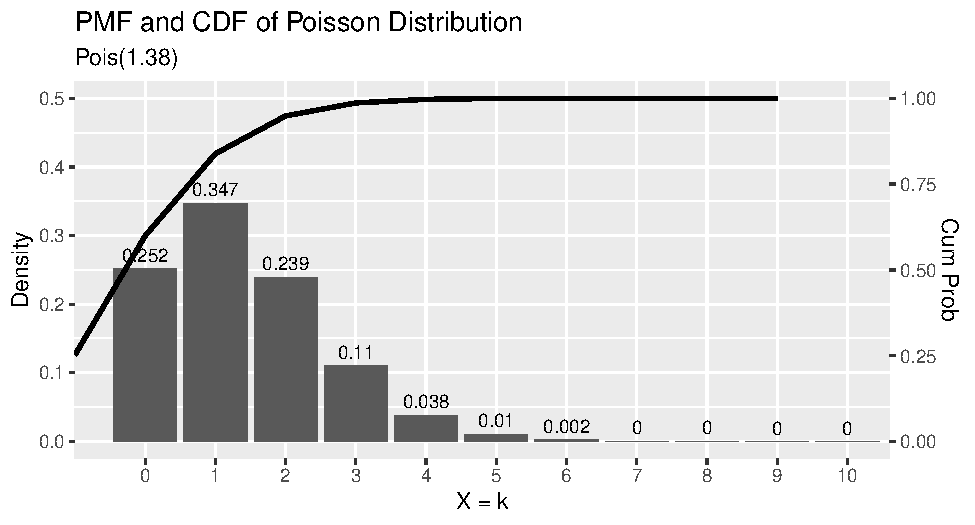
\includegraphics{probability_files/figure-latex/unnamed-chunk-22-1.pdf}

How well does the Poisson distribution fit the 2002 World Cup data?

\begin{Shaded}
\begin{Highlighting}[]
\NormalTok{dat }\OperatorTok
\StringTok{  }\KeywordTok{mutate}\NormalTok{(}\DataTypeTok{pred =}\NormalTok{ n }\OperatorTok{*}\StringTok{ }\KeywordTok{dpois}\NormalTok{(}\DataTypeTok{x =}\NormalTok{ goals, }\DataTypeTok{lambda =}\NormalTok{ lambda)) }\OperatorTok
\StringTok{  }\KeywordTok{rename}\NormalTok{(}\DataTypeTok{obs =}\NormalTok{ freq) }\OperatorTok
\StringTok{  }\KeywordTok{pivot_longer}\NormalTok{(}\DataTypeTok{cols =} \OperatorTok{-}\NormalTok{goals) }\OperatorTok
\StringTok{  }\KeywordTok{ggplot}\NormalTok{(}\KeywordTok{aes}\NormalTok{(}\DataTypeTok{x =}\NormalTok{ goals, }\DataTypeTok{y =}\NormalTok{ value, }\DataTypeTok{color =}\NormalTok{ name)) }\OperatorTok{+}
\StringTok{  }\KeywordTok{geom_point}\NormalTok{() }\OperatorTok{+}
\CommentTok{#  geom_smooth(se = FALSE) +}
\StringTok{  }\KeywordTok{theme}\NormalTok{(}\DataTypeTok{legend.position =} \StringTok{"top"}\NormalTok{) }\OperatorTok{+}
\StringTok{  }\KeywordTok{labs}\NormalTok{(}
    \DataTypeTok{title =} \StringTok{"Poisson Dist: Observed vs Expected"}\NormalTok{,}
    \DataTypeTok{color =} \StringTok{""}\NormalTok{,}
    \DataTypeTok{y =} \StringTok{"frequencey"}
\NormalTok{  )}
\end{Highlighting}
\end{Shaded}

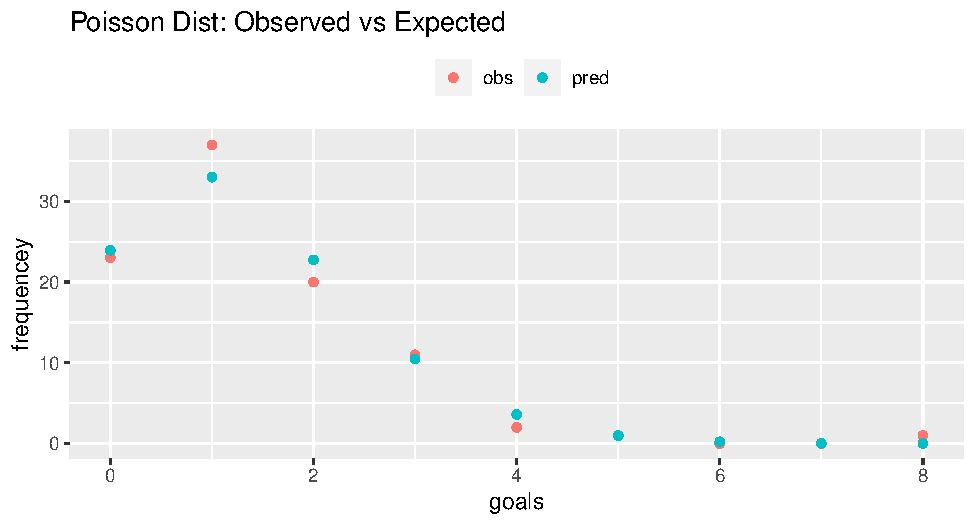
\includegraphics{probability_files/figure-latex/unnamed-chunk-23-1.pdf}

It seems to fit pretty good! You can run a chi-square goodness-of-fit test to confirm. The test requires an expected frequency of at least 5 per cell. Cells 4 through 8 are under 5, so you need to lump them.

\begin{Shaded}
\begin{Highlighting}[]
\NormalTok{x <-}\StringTok{ }\NormalTok{dat }\OperatorTok\StringTok{ }
\StringTok{  }\KeywordTok{group_by}\NormalTok{(}\DataTypeTok{goals =} \KeywordTok{if_else}\NormalTok{(goals }\OperatorTok{>=}\StringTok{ }\DecValTok{4}\NormalTok{, }\DecValTok{4}\NormalTok{, goals)) }\OperatorTok\StringTok{ }
\StringTok{  }\KeywordTok{summarize}\NormalTok{(}\DataTypeTok{.groups =} \StringTok{"drop"}\NormalTok{, }\DataTypeTok{freq =} \KeywordTok{sum}\NormalTok{(freq)) }\OperatorTok\StringTok{ }
\StringTok{  }\KeywordTok{pull}\NormalTok{(freq)}
\NormalTok{p <-}\StringTok{ }\NormalTok{dat }\OperatorTok\StringTok{ }
\StringTok{  }\KeywordTok{mutate}\NormalTok{(}\DataTypeTok{p =} \KeywordTok{dpois}\NormalTok{(}\DataTypeTok{x =}\NormalTok{ goals, }\DataTypeTok{lambda =}\NormalTok{ lambda)) }\OperatorTok
\StringTok{  }\KeywordTok{group_by}\NormalTok{(}\DataTypeTok{goals =} \KeywordTok{if_else}\NormalTok{(goals }\OperatorTok{>=}\StringTok{ }\DecValTok{4}\NormalTok{, }\DecValTok{4}\NormalTok{, goals)) }\OperatorTok\StringTok{ }
\StringTok{  }\KeywordTok{summarize}\NormalTok{(}\DataTypeTok{.groups =} \StringTok{"drop"}\NormalTok{, }\DataTypeTok{p =} \KeywordTok{sum}\NormalTok{(p)) }\OperatorTok\StringTok{ }
\StringTok{  }\KeywordTok{pull}\NormalTok{(p)}
\NormalTok{(chisq_test <-}\StringTok{ }\KeywordTok{chisq.test}\NormalTok{(}\DataTypeTok{x =}\NormalTok{ x, }\DataTypeTok{p =}\NormalTok{ p, }\DataTypeTok{rescale.p =} \OtherTok{TRUE}\NormalTok{))}
\end{Highlighting}
\end{Shaded}

\begin{verbatim}
## 
##  Chi-squared test for given probabilities
## 
## data:  x
## X-squared = 1.0414, df = 4, p-value = 0.9035
\end{verbatim}

\begin{center}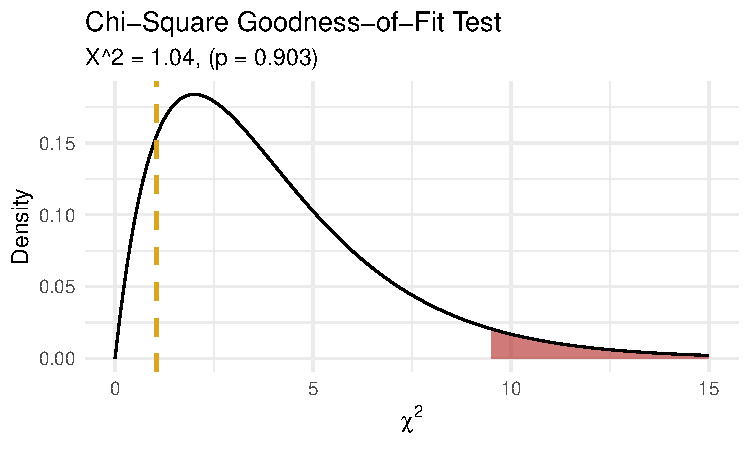
\includegraphics{probability_files/figure-latex/unnamed-chunk-25-1} \end{center}

\begin{quote}
A chi-square goodness-of-fit test was conducted to determine whether the matches had the same proportion of goals as the theoretical Poisson distribution. The minimum expected frequency was 5. The chi-square goodness-of-fit test indicated that the number of matches with 0, 1, 2, 3, or 4 or more goals was \emph{not} statistically significantly different from the proportions expected in the theoretical Poisson distribution (\(X^2\)(4) = 1.041, \emph{p} = 0.903).
\end{quote}

As demonstrated above, the \(\mathrm{Pois}(\lambda)\) approaches the \(\mathrm{Bin}(n, \pi)\) where \(n\pi = \lambda\) when \(n \rightarrow \infty\) and \(\pi \rightarrow 0\). The Poisson is a useful (computationally inexpensive) approximation to the binomial when (\(n \ge 20\)) and \(\pi \le 0.05\)). For example, suppose a baseball player has a \(\pi = .03\) chance of hitting a home run. What is the probability of hitting \(X \ge 20\) home runs in \(n = 500\) at-bats? This is a binomial process because the sample size is fixed.

\begin{Shaded}
\begin{Highlighting}[]
\KeywordTok{pbinom}\NormalTok{(}\DataTypeTok{q =} \DecValTok{20}\NormalTok{, }\DataTypeTok{size =} \DecValTok{500}\NormalTok{, }\DataTypeTok{prob =} \FloatTok{0.03}\NormalTok{, }\DataTypeTok{lower.tail =} \OtherTok{FALSE}\NormalTok{)}
\end{Highlighting}
\end{Shaded}

\begin{verbatim}
## [1] 0.07979678
\end{verbatim}

But \(n\) is large and \(\pi\) is small, so the Poisson distribution works well too.

\begin{Shaded}
\begin{Highlighting}[]
\KeywordTok{ppois}\NormalTok{(}\DataTypeTok{q =} \DecValTok{20}\NormalTok{, }\DataTypeTok{lambda =} \FloatTok{0.03} \OperatorTok{*}\StringTok{ }\DecValTok{500}\NormalTok{, }\DataTypeTok{lower.tail =} \OtherTok{FALSE}\NormalTok{)}
\end{Highlighting}
\end{Shaded}

\begin{verbatim}
## [1] 0.08297091
\end{verbatim}

\begin{Shaded}
\begin{Highlighting}[]
\NormalTok{n =}\StringTok{ }\DecValTok{500}
\NormalTok{p =}\StringTok{ }\FloatTok{0.03}
\NormalTok{x =}\StringTok{ }\DecValTok{0}\OperatorTok{:}\DecValTok{30}
\KeywordTok{data.frame}\NormalTok{(}
  \DataTypeTok{events =}\NormalTok{ x, }
  \DataTypeTok{Poisson =} \KeywordTok{dpois}\NormalTok{(}\DataTypeTok{x =}\NormalTok{ x, }\DataTypeTok{lambda =}\NormalTok{ p }\OperatorTok{*}\StringTok{ }\NormalTok{n),}
  \DataTypeTok{Binomial =} \KeywordTok{dbinom}\NormalTok{(}\DataTypeTok{x =}\NormalTok{ x, }\DataTypeTok{size =}\NormalTok{ n, }\DataTypeTok{p =}\NormalTok{ p)}
\NormalTok{) }\OperatorTok
\StringTok{  }\KeywordTok{pivot_longer}\NormalTok{(}\DataTypeTok{cols =} \OperatorTok{-}\NormalTok{events) }\OperatorTok
\StringTok{  }\KeywordTok{ggplot}\NormalTok{(}\KeywordTok{aes}\NormalTok{(}\DataTypeTok{x =}\NormalTok{ events, }\DataTypeTok{y =}\NormalTok{ value, }\DataTypeTok{color =}\NormalTok{ name)) }\OperatorTok{+}
\StringTok{  }\KeywordTok{geom_line}\NormalTok{() }\OperatorTok{+}
\StringTok{  }\KeywordTok{theme}\NormalTok{(}\DataTypeTok{legend.position =} \StringTok{"top"}\NormalTok{) }\OperatorTok{+}
\StringTok{  }\KeywordTok{labs}\NormalTok{(}\DataTypeTok{title =} \StringTok{"Pois(.03*500) vs. Bin(500, .03)"}\NormalTok{,}
       \DataTypeTok{subtitle =} \StringTok{"Poisson approximation to binomial."}\NormalTok{,}
       \DataTypeTok{x =} \StringTok{"Events"}\NormalTok{,}
       \DataTypeTok{y =} \StringTok{"Density"}\NormalTok{,}
       \DataTypeTok{color =} \StringTok{""}\NormalTok{)}
\end{Highlighting}
\end{Shaded}

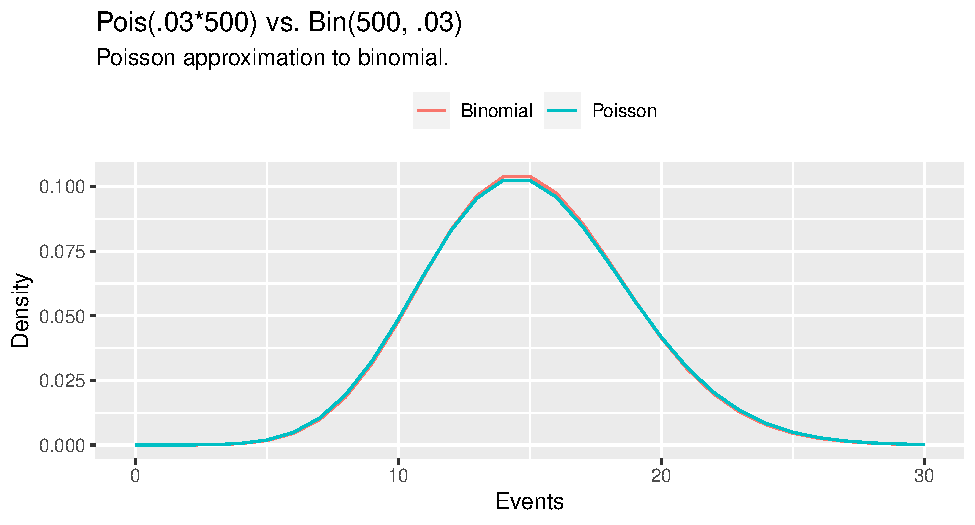
\includegraphics{probability_files/figure-latex/unnamed-chunk-28-1.pdf}

When the observed variance is greater than \(\lambda\) (overdispersion), the Negative Binomial distribution can be used instead of Poisson.

\hypertarget{exponential}{%
\section{Exponential}\label{exponential}}

\hypertarget{gamma}{%
\section{Gamma}\label{gamma}}

The gamma distribution shows up primarily in models of wait times until events. Unlike the exponential distribution which models the time until the first event, gamma models the time until the \(k\)th event.

Before you learn about the gamma distribution, you should understand the gamma \emph{function} because it is part of the definition.

\[\Gamma(n) = (n-1)!\]

extends the factorial for nonnegative whole numbers to a larger subset of the real numbers.

The generalization of the factorial is used in combinatorics and probability problems. Some probability distributions are defined in terms of the gamma function, including the student t, chi-square, and gamma distribution.

The gamma distribution is a two-parameter distribution. You will encounter two forms of the gamma distribution.

\begin{itemize}
\tightlist
\item
  \textbf{shape} \(k\) and \textbf{scale} \(\theta\).
\item
  \textbf{shape} \(\alpha = k\) and \textbf{rate} \(\beta = 1/\theta\).
\end{itemize}

The probability density function for the shape \(k\) and scale \(\theta\) form is

\[f(x; k, \theta) = \frac{x^{k-1} e^{-\frac{x}{\theta}}}{\theta^k \Gamma(k)} \hspace{1cm} x, k, \alpha, \beta > 0.\]

The probability density function for the shape \(\alpha\) and rate \(\beta\) form is

\[f(x; \alpha, \beta) = \frac{\beta^\alpha x^{\alpha-1}e^{-\beta x}}{\Gamma(k)} \hspace{1cm} x, \alpha, \theta > 0.\]

In a time-to-event application, \(\alpha\) represents the event number and \(\beta\) the event rate.

It is the conjugate prior to the Poisson, exponential, normal, Pareto, and gamma likelihood distributions.

The gamma distribution can be used to model the interval of time between earthquakes.

References: \href{https://towardsdatascience.com/gamma-distribution-intuition-derivation-and-examples-55f407423840}{Arein Kim}.

\hypertarget{beta}{%
\section{Beta}\label{beta}}

The beta distribution, \(\mathrm{Beta}(\alpha, \beta)\), is a family of continuous probability distributions defined on the interval {[}0, 1{]} and parameterized by two positive shape parameters, \(\alpha\) and \(\beta\). The Dirichlet distribution generalizes the beta distribution to multiple variables.

In Bayesian inference, the beta distribution is the conjugate prior probability distribution for the Bernoulli, binomial, negative binomial and geometric distributions. The beta distribution is a good model for proportions.

The probability density function is

\[f(x; \alpha, \beta) = \]

\hypertarget{methods}{%
\chapter{Methods}\label{methods}}

We describe our methods in this chapter.

\hypertarget{applications}{%
\chapter{Applications}\label{applications}}

Some \emph{significant} applications are demonstrated in this chapter.

\hypertarget{example-one}{%
\section{Example one}\label{example-one}}

\hypertarget{example-two}{%
\section{Example two}\label{example-two}}

\hypertarget{bayesian-inference}{%
\chapter{Bayesian Inference}\label{bayesian-inference}}

To be amenable to analysis, \emph{all} uncertainties need to be described by probabilities.

\hypertarget{prior-and-posterior-distributions}{%
\section{Prior and Posterior Distributions}\label{prior-and-posterior-distributions}}

The Bayesian model for inference contains the statistical model \({f_\theta: \theta \in \Omega}\) for the data \(s \in S\) and adds to this the prior probability measure \(\Pi\) for \(\theta\). \({f_\theta: \theta \in \Omega}\) is a conditional distribution for \(s\) given \(\theta\). For example, if \(\theta\) is the probability of a coin landing on heads with \(\Omega = [0,1]\), then the prior density \(\pi\) would be some sort of bell curve around \(\theta = 0.5\).

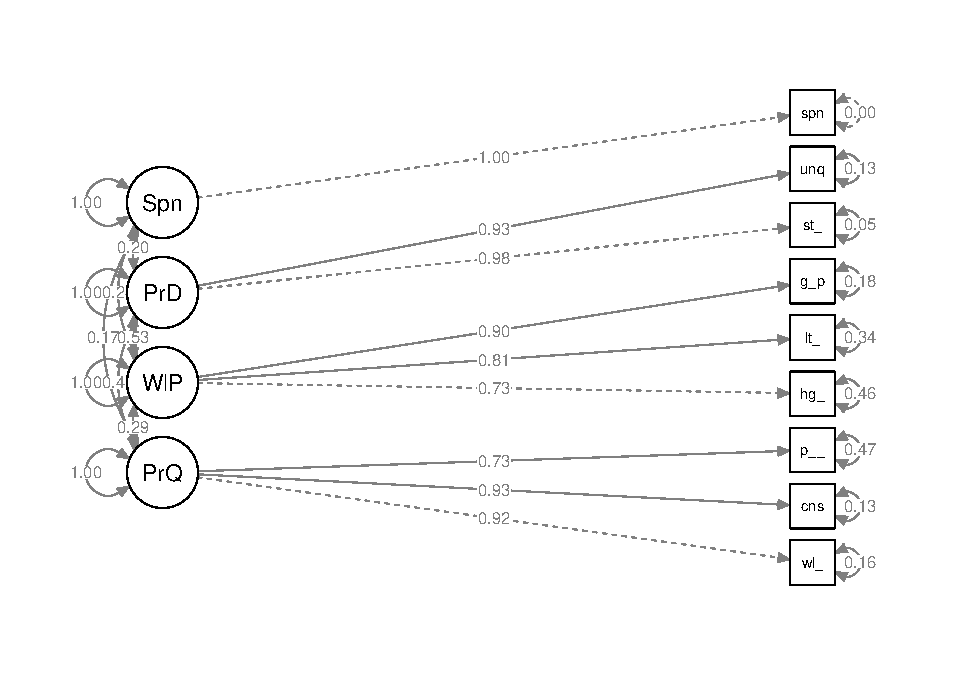
\includegraphics{probability_files/figure-latex/unnamed-chunk-30-1.pdf}

By the law of total probability, the prior and conditional probability constitute a joint distribution for \((s, \theta)\), \(\pi(\theta)f_\theta(s)\) where \(\pi\) is the probability function associated with \(\Pi\). For continuous distributions, the marginal distribution of \(s\), called the \emph{prior predictive distribution} is

\[m(s) = \int_\Omega \pi(\theta)f_\theta(s) d\theta\]

After observing data, the relevant distribution is the conditional probability, \(\Pi(\cdot|s)\), or \emph{posterior distribution}. The posterior density is the joint density divided by the marginal density.

\[\pi(\theta|s) = \frac{\pi(\theta)f_\theta(s)}{m(s)}\]

\hypertarget{example-bernoulli-model}{%
\subsubsection*{Example: Bernoulli Model}\label{example-bernoulli-model}}
\addcontentsline{toc}{subsubsection}{Example: Bernoulli Model}

Suppose you observe a sample \((x_1, \ldots, x_n)\) from the \(\mathrm{Bernoulli}(\theta)\) with unknown \(\theta \in [0,1]\). For the prior, take \(\pi\) to be a \(\mathrm{Beta}(\alpha,\beta)\) density function \(\frac{1}{\mathrm{B}(\alpha,\beta)} x^{\alpha-1}(1-x)^{\beta-1}\). Then the posterior of \(\theta\) is proportional to the likelihood \(\Pi_{i=1}^n \theta^{x_i} (1-\theta)^{1-x_i} = \theta^{n\bar{x}}(1-\theta)^{n(1-\bar{x})}\) multiplied by the prior.

  \bibliography{book.bib,packages.bib}

\end{document}
